\documentclass[a4paper]{article}

\usepackage[english]{babel} \usepackage[utf8x]{inputenc}
\usepackage{amsmath}
\usepackage{graphicx}
\usepackage[colorinlistoftodos]{todonotes} \usepackage[margin = 1.2in]{geometry}

\title{A Bug's Life\\
 Operating systems and process-oriented programming (1DT096), project proposal
, group 5}
\date{\today}
\author{Oliver Eriksson Edholm (930615-5210) \\
Aleksander Lundqvist (900728-0317) \\
Henrik Sommerland (890618-4950) \\
Edvin Wahlberg (910721-3176) \\
Oscar Wallster(910615-1096)}


\begin{document}
\maketitle

\section{Introduction}
% This could be rewritten in a far more persuasive manner
We have decided that we are going to simpulate an \emph{ant ant}. We want to do
this in order to learn more about both \emph{swarm intelligence} and the actor
model.\\
We choose ants in inspiration of their ability to cooperate in a very large
scale and solve complex problems while still every ant is only following very
simple set of rules.

Our goal is not to simulate the behaviour of real world ants or to mimic the
datails of any biological systems.
We are more interested in the theorethical concepts of how complex behaviors can
arise from the interaction of a large group of agents each possessing only limited
cognitive abilites.\\

One of the later goals is also to have two or more ant hives interact with
eachother in a world where food is scarce, and battles are inevitable.

\subsection{Challenges}
During the course of this project we are aware that there may be many challenges
ahead.

\subsubsection{Technical Challenges}
Making heavy use of the actor model using thousands of actors will create a lot
of complexity and there are many posibilities for problems to occur. The most
obvious danger is the possibilty of deadlocks to occur. With many actors
communicating together one is almost certain that one will get some form of
circular dependency. So great care needs to be taken to ensure that no
deadlocks will occur.

There is also a risk of severe performance degradation in regions with many
interacting actors. Although this is something wich is intrinsic to the actor
model and it may be hard for us to control.

\subsubsection{Rules For Interaction}
The other challenge will be to set up rules for how the ants interact with the
world and how the world gets updated. The parameters for these rules will need
to be finetuned and it may be hard to find rules which result in complex
behaviours. It is also very hard to analytically determine these parameters so
the only feasible alternative is to trough experimentation find rules which
yields satisfactory behaviours.

\subsubsection{Social Challenges}
In order to get this project moving forward in a pace that is required, we need
to have every member of the group working regularly certain hours of the weeks.
In order to achieve this every member needs to have the same mental image over
the finished project, therefore we need to be active with communication in the
group so that no one is left behind and wonders what he could/should be doing.

\section{Concurrency Models and Programming Languages}
This section will contain our thoughts on what form of concurrency we want to
use and what languages will be apropriate.
\subsection{Concurrency Goals}
As previously stated we want to create a system wich relies heavily on the actor
model. Our project idea is well suited for this since the ants are by nature
individual agents who and make decisions without any direct knowlegde of the
global state.

We want to make our simulation free of so called \emph{stop the world}
sencarios. These are when we for some reason have to block all of the actors in
the simulation in order to perform some kind of action.

\subsection{Language Requirement}
Our main requirement for the programming language we choose is that it have to meet our concurency goals.
We have discarded c/c++ because it's to lowlevel and we would have to implement the actor model ourselves or make us of a library we know nothing of. 
Also java because it's not the proper concurrency model. We are considering python for frontend(graphics),
but it's not suited for our backend needs.

\subsection{Rust}
Rust is a very compelling language for this project. Built for concurrency, fully realised
actor model and really fast. Sadly, it is quite difficult to do very basic things and the need
of understanding the ownership model used in Rust will mean that a lot of time will be wasted
on things that do not bring the project forward. 

\subsection{Nim}
Nim has a very nice and simple Python-esque syntax, and has surprising performance due to it
transpiling to C before compilation. It has a actor model like take on threads, with message
passing between them, and also a proper actor model in its standard library. It is however a
very young language (v 0.1 at time of writing) with a large amount of compiler bugs. It is
unknown how it would handle the massive concurrency that is needed for this project. 

\subsection{Erlang}
Built for massive concurrency and is the text book example of the actor model. Also extremely
low thread-by-thread performance, and blocking receives for messages means extra work in
trying to get around some problems that will be relevant in this project. 

\subsection{Encore}
Encore would be a great language for this project since encore is completley
built on the actor model. The problem with encore is that it is in its pre
alpha stage and thus its not a viable option for this project.

\section{System Architecture}
\begin{figure}[h!]
\centerline{
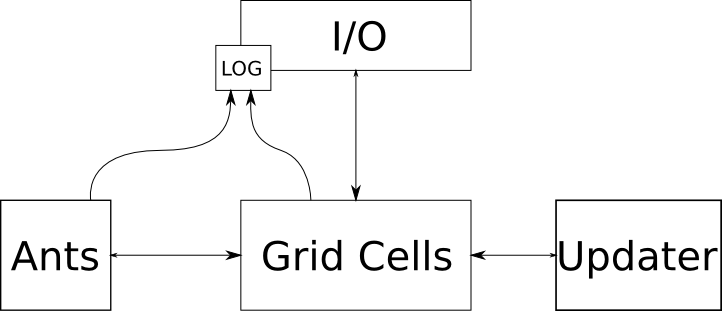
\includegraphics[scale=0.6]{images/architecture.png} 
}
\caption{A draft of a system architecture} 
\label{fig:arch}
\end{figure}

Above you can see a rough draft of the architecture of the system. Each box
represents an agent, note that this is just a conceptual map of the
communication between the different agents. The arrows between the a means that
they comunicate via message passing.
The large arrow indicates that a message will be sent between those actors in that
direction. The smaller arrows on the lines indicates that the sending actor
will block until a reply message is received.

\subsection{Ants}
In figure~\ref{fig:arch} the box labled \textbf{Ants} corresponds to the ant
object.
The ant will be an independent actor holding very little information about its
own state but containing the faculties to make decisions based on received
input. The ant actor will send a message to the cell querying about the state
of its neighbouring cells. The ant will then wait for the reply message from its
cell and then take some action based on the reply from the cell. the actor then
sends a message to its cell requesting to do whatever it is that the ant wanted
to do and then awaits a reply whether or not the move was successfull.

\subsection{Grid Cell}
In figure~\ref{fig:arch} the box labled \textbf{Grid Cells} corresponds to one
cell on the ``map''. Each of these cells contains all the information about the state of
that cell. It also contains references to its neighbouring cells in order to
retrive the information about its neighbourhood. The cell will wait for queries
from ants to receive the state of the neighbourhood and the cell will also
process requests from ants to perform actions such as moving or picking up food.

\subsection{Updater}
In figure~\ref{fig:arch} the box labled \textbf{Updater} is something that will
handle the background work for the cells. Such as the dissipation of the pheromones.
We are uncertain whether or not to use this approach with a separate actor sweeping
trough all of the cells and updating them. We could let each of the cells handle
their own ``passive'' updates but that might result in performance degradation
since the cells would either always be doing work or we might need to introduce
some form of delay.

\subsection{I/O}
In figure~\ref{fig:arch} the box labled \textbf{I/O} is the actor that be
responsible for the handling of the input and output. This actor will sweep thrugh the cells and
query them for their state and then process output the information in some
suitable fashion. We may add support for some form of interactivity at a later
state.

\subsection{LOG}
In figure~\ref{fig:arch} the box labled \textbf{LOG} will be a simple actor wich
is just waiting for logging mesages from the ants and the grid cells. This will be
used as a form of rudimentary output and for debugging purposes.


\section{Development Tools}
Below there will folow a short discussion about what tools we decided to use.
\subsection{Communication and planning}
To plan meetings and set up to-do tasks
for the project, we have chosen to use Trello. Trello is a very user friendly and will
give us a great overview of the progress of the project. It will also be a good
tool to keep track of who is doing what. For communication we’re going to use
Slack to ensure that we have all communication of the project in one place. If
we should have chosen to use Facebook it’s very easy to get distracted and talk
about other things that isn’t related to the project. If we really need to discuss
something urgent we’re going to use Skype.Working in a group of six fully active members
it is very important that everyone in the group keeps himself up-to-date with the progress. 
We were therefore very carefull when choosing the communication medias so that everyone would
feel that they would check the media every day. Again, the problem with facebook is that 
although everyone would check it daily, there would be a lot of other things going on.
The communication environment needs to be strictly for work related things to keep everyone
focused on what's important.

\subsection{Development}
We will be using GitHub for source control. We will try to keep track of all
issues using GitHubs issue tracking system. We will make no restrictions or
requirements of what IDE/editor to be used.\\
Since we have not choosen our language yet we are not shure what build tools we
will use. That descision is based upon what languages we will use.



\section{Conclusion}
Digital ant colonization is perfect project for developing deeper understanding
of the actor model of concurency, since each ant is an independent actor and
only interact with its immidiate surroundings. This project can be divided into
different milestones which can be developed further as time goes on. We all have
alot and diffrent ideas how we want the final product to work, but we all agree
on the basics so as time elapse we will hopefully be able to add alot more
complexity depending how much work will be needed for each milestone. Ergo we
start with a stable core and build outwards in different directions.
\end{document}

